\chapter{Алгоритмы на графах}
\section{Алгоритм Флойда-Уоршела}
\subsection{Описание алгоритма}
\textbf{Задача алгоритма:} \emph{нахождение кратчайших расстояний между всеми вершинами взвешенного ориентированного графа.}

Алгоритм: на каждом шаге проверяем новое количество вершин, т.е. на первом шаге имеем путь между двумя соседними вершинами --- ребро, соединяющее вершины. На втором шаге выбираем какую-то вершину и смотрим, будет ли короче путь между двумя изначальными вершинами, если пройти через эту выбранную точку. Далее выбираем следующую точку и т.д. Таким образом мы постепенно исследуем все пути из вершины в вершину через постепенно растущее число вершин. 

Строим последовательность матриц (методом динамического программирования) $a_{ij}^0 \rightarrow a^1_{ij} \rightarrow a^2_{ij} \rightarrow\dots\rightarrow a^n_{ij}$. $a^k_{ij}$ --- кратчайшее расстояние от i-ой до j-ой вершины, при этом как промежуточными пользуемся от 1-ой до k-ой.\\
$a_{ij}^0 = W_{ij}$ --- промежуточными вершинами пользоваться нельзя.\\
Правило поиска следующей матрицы: $a_{ij}^k= \min(a^{k-1}_{ij}, a^{k-1}_{ik}+a^{k-1}_{kj}).$\\
Сложность алгоритма: $O(N^3)$.

Более подробно алгоритм описан в \href{https://ru.wikipedia.org/wiki/%D0%90%D0%BB%D0%B3%D0%BE%D1%80%D0%B8%D1%82%D0%BC_%D0%A4%D0%BB%D0%BE%D0%B9%D0%B4%D0%B0_%E2%80%94_%D0%A3%D0%BE%D1%80%D1%88%D0%B5%D0%BB%D0%BB%D0%B0}{википедии}.
\subsection{Реализация}
Будем запоминать все предыдущие матрицы (что необязательно).

\begin{infa}{Реализация алгоритма Флойда-Уоршела}
\num A = [[[INF]*n \fori i \ini \rangei(n)] \fori k \ini \rangei(n+1)] \com{INF - условная\\\phantom{6\ \ \ \ }бесконечность, n - число ребер}
\num \fori i \ini \rangei(n):
\num \tab A[0][i][:] = W[i] \com{При копировании весовой матрицы W расстояние от вершины\\\phantom{6\ \ \ \ }до себя равно нулю; забиваем матрицу рёбер т.е. расстояния в начальный момент.}
\num \fori k \ini \rangei(1, n+1):
\num \tab \fori i \ini \rangei(n):
\num \tab \tab \fori j \ini \rangei(n):
\num \tab \tab \tab A[k][i][j] = \mini(A[k-1][i][j], A[k-1][i][k]+A[k-1][k][j]) \com{Добав-\\\phantom{6\ \ \ \ }ляем путь от i до j вершины через новую вершину, если такой путь короче}
\end{infa}
Алгоритм не работает с циклами отрицательного веса, т.к. можно <<накрутить>> минус бесконечность. Но если при этом путь от i-ой до j-ой вершины не содержит такого цикла, то алгоритм сработает правильно.
\section{Топологическая сортировка}
Если граф не содержит циклов, то его вершины можно пронумеровать так, что любое ребро идет от вершины с меньшим номером к вершине с большим номером.

\textsf{Топологическая сортировка} — упорядочивание вершин бесконтурного ориентированного графа согласно частичному порядку, заданному ребрами орграфа на множестве его вершин.

Т.е. если граф не содержит циклов, то его вершины можно пронумеровать так, что любое ребро идет от вершины с меньшим номером к вершине с большим номером.\\
Применяется в различных прикладных задачах. 

\subsection{Алгоритм Кана}
\noindent A(k) --- множество вершин, от которых <<зависит>> вершина k (т.е. в которую можно прийти от других вершин).\\P --- последовательность вершин.\\
Алгоритм:\\
\texttt{Пока \abs{P} < N:\\
\phantom{\tab }Найти вершину v, у которой A(v) = $\varnothing$ \\%пустое множество
\phantom{\tab }P.append(v)\\
\phantom{\tab }Вычеркнуть v из всех множеств A(k).\\}
Алгоритм очень громоздкий и неэффективный.
\subsection{Алгоритм Тарьяна}
\subsubsection{Алгоритм}
Сложность алгоритма: $O(n)$.\\
По факту мы просто осуществляем обход в глубину, в котором мы будем красить вершины.\\
\textsf{Подход алгоритма:} DFS с покраской вершин (белая/серая/черная).\\
С любой вершины не used вершины запускаем DFS. Белые вершины --- еще не тронутые, серые вершины --- те, в которые алгоритм вошел, черные вершины --- те, из которого алгоритм вышел.\\
Попытка входа в серую вершины означает наличие цикла, значит алгоритм невозможен.
При выходе из вершины (в момент покраски ее в черный цвет) добавляем ее в начало списка.

\subsubsection{Реализация алгоритма}
\begin{infa}{Реализация алгоритма Тарьяна}
	\ \num Visited = [\Falsei]*(n + 1)
	\ \num Ans = []
	\ \num 
	\ \num \defi DFS(start):
	\ \num \tab Visited[start] = \Truei
	\ \num \tab \fori u \ini V[start]:
	\ \num \tab \tab \ifi \noti Visited[u]:
	\ \num \tab \tab \tab DFS(u)
	\ \num \tab Ans.append(start)
	\num
	\num \fori i \ini \rangei(1, n + 1): 
	\num \tab \ifi \noti Visited(i): 
	\num \tab \tab DFS(i) 
	\num Ans = Ans[::-1]
\end{infa}
%рисунок 2
%реализации не будет
\section{Неэффективные алгоритмы}
\subsection{Задача Коммивояжера}
\textbf{Задача:} \emph{найти минимальный по весу гамильтонов цикл. Сложность алгоритма: $O(N!)$.}

В графе есть вершины. Коммивояжер захотел посетить  все эти вершины и вернутся домой. Гамильтонов цикл точно есть в этой системе (это легко проверить, соединив все вершины по порядку). То есть, задача сводится к тому, чтобы найти минимальный по весу Гамильтонов цикл. Но эта задача плохо реализуется при большом числе вершин, так как основа решения --- перебор. Т.е. имеем $N!$ потенциально возможных гамильтоновых циклов, каждый имеет свой вес.

К примеру, на рис. \ref{ris1} изображен оптимальный маршрут коммивояжёра через 15 крупнейших городов Германии. Указанный маршрут является самым коротким из всех возможных 43 589 145 600 вариантов.
\begin{figure}[h!]
	\centering
	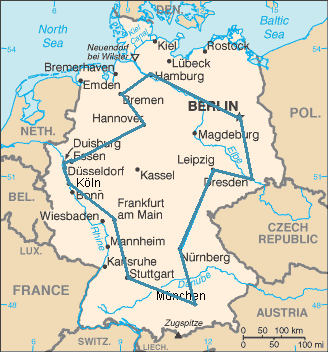
\includegraphics[width=0.5\linewidth]{lection_21/germany}
	\caption{Оптимальный маршрут коммивояжёра через 15 крупнейших городов Германии}
	\label{ris1}
\end{figure}

Таким образом оптимизировать эту задачу невозможно.

%рис 3, нужно доехать из A в B и посетить все пункты
\subsection{Задача о китайском почтальоне}
%рис 4
\textbf{Задача:} \emph{пройти по каждому ребру графа минимум 1 раз, чтобы доставить почту. Требуется найти такой цикл минимального суммарного веса.}

То есть, нам необходимо найти цикл минимального суммарного веса, такой, что он проходит по ребру хотя бы 1 раз. Важное замечание --- если граф Эйлеров, то Эйлеров цикл и есть решение этой задачи. А вот если его нет, то задача усложняется --- решение можно найти только полным перебором. Итоговый алгоритм получается неэффективным, т.к. его асимптотика $O(N!)$.